%%%%%%%%%%%%%%%%%%%%%%%%%%%%%%%%%%%%%%%%%
% Tutorial
% LaTeX Template
% Version 1.0 (05/11/17)
%
% Author:
% Ben Roose (ben.roose@wichita.edu)
%
% Original template author:
% Adam Glesser (adamglesser@gmail.com)
% www.LaTeXTemplates.com
%
% License:
% CC BY-NC-SA 3.0 (http://creativecommons.org/licenses/by-nc-sa/3.0/)
%
%%%%%%%%%%%%%%%%%%%%%%%%%%%%%%%%%%%%%%%%%

\documentclass[12pt]{article}

\usepackage{graphicx} %Allow import of images
\graphicspath{ {images/} } % Relative path to images directory
\usepackage[margin=1in]{geometry} % Required to make the margins smaller to fit more content on each page
\usepackage[linkcolor=blue]{hyperref} % Required to create hyperlinks to questions from elsewhere in the document
\hypersetup{pdfborder={0 0 0}, colorlinks=true, urlcolor=blue} % Specify a color for hyperlinks
\usepackage{todonotes} % Required for the boxes that questions appear in
\usepackage{tocloft} % Required to give customize the table of contents to display questions
\usepackage{microtype} % Slightly tweak font spacing for aesthetics
\usepackage{palatino} % Use the Palatino font

\setlength\parindent{0pt} % Removes all indentation from paragraphs

% Create and define the list of questions
\newlistof{questions}{faq}{\large FAQ for accessing the Routing \& Switching Lab in EE 328C and 328D} % This creates a new table of contents-like environment that will output a file with extension .faq
\setlength\cftbeforefaqtitleskip{3em} % Adjusts the vertical space between the title and subtitle
\setlength\cftafterfaqtitleskip{1em} % Adjusts the vertical space between the subtitle and the first question
\setlength\cftparskip{.3em} % Adjusts the vertical space between questions in the list of questions

% Create the command used for questions
\newcommand{\question}[1] % This is what you will use to create a new question
{
\refstepcounter{questions} % Increases the questions counter, this can be referenced anywhere with \thequestions
\par\noindent % Creates a new unindented paragraph
\phantomsection % Needed for hyperref compatibility with the \addcontensline command
\addcontentsline{faq}{questions}{#1} % Adds the question to the list of questions
\todo[inline, color=green!40]{\textbf{#1}} % Uses the todonotes package to create a fancy box to put the question
\vspace{1em} % White space after the question before the start of the answer
}

% Uncomment the line below to get rid of the trailing dots in the table of contents
%\renewcommand{\cftdot}{}

% Uncomment the two lines below to get rid of the numbers in the table of contents
%\let\Contentsline\contentsline
%\renewcommand\contentsline[3]{\Contentsline{#1}{#2}{}}

\begin{document}

%----------------------------------------------------------------------------------------
%	TITLE AND LIST OF QUESTIONS
%----------------------------------------------------------------------------------------

\begin{center}
\Huge{\bf \emph{EECS Tutorial: Routing \& Switching Lab}} % Main title
\end{center}

\listofquestions % This prints the subtitle and a list of all of your questions
\bigskip % Create a gap between list and first question

%\newpage % Comment this if you would like your questions and answers to start immediately after table of questions

%----------------------------------------------------------------------------------------
%	QUESTIONS AND ANSWERS
%----------------------------------------------------------------------------------------
\begin{flushleft}

\question{What is the default login username and password for Arista switches?}\label{password}

\begin{verbatim}
Username: student
Password: arista
\end{verbatim}

\newpage
%------------------------------------------------

\question{How do I access rslab equipment from a mobile Linux terminal in EE 328C?}\label{mobile_terminals}

\begin{enumerate}
  \item In EE 328C turn on a mobile Linux terminal. Computer will network boot from the rslab LTSP server and automatically log into a GUI desktop environment.
  \item Open \textit{PAC Manager} from the Desktop or the \textit{applications} menu.
  \item On left side, double-click the terminal server for the rack \# assigned to you by GTA. A new session tab window will open and connect into the terminal server.
  \item Once connected to the terminal server for your assigned rack, use the menu to connect/disconnect the Arista switches and Cisco router in the networking rack.
  \item You can return to the terminal server menu by pressing \texttt{CTRL+SHIFT+7}.
  \item To view all open connections in the session, return to the menu and press \texttt{16}.
  \item To exit from the terminal server, return to the menu and press \texttt{18}.
\end{enumerate}

\textbf{NOTE:} You can open more than one tabbed session within \textit{PAC Manager} to access the same rack terminal server and connect to multiple network devices concurrently, but each switch or router can only be accessed by one terminal server session at a time.

\begin{figure}[h]
  \caption{Example of connecting with \textit{PAC Manager} from a mobile Linux terminal}
  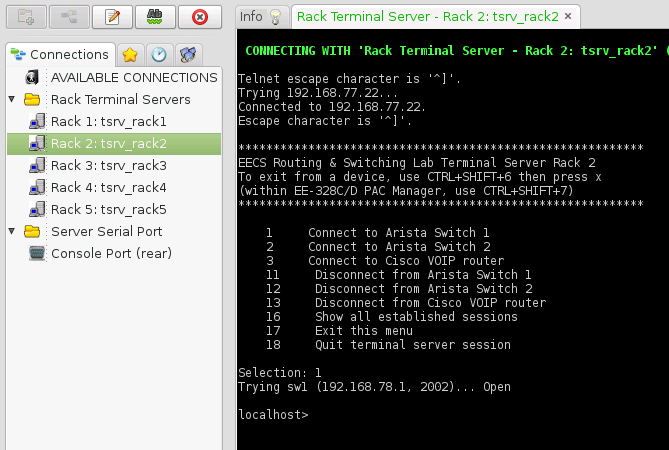
\includegraphics[width=.9\linewidth]{rslab_pac}
  \centering
\end{figure}

\newpage
%------------------------------------------------

\question{How do I access rslab equipment using a computer in EE 327 or EE 328 labs?}\label{remote_access}

\begin{enumerate}
  \item Run the SSH \textit{PuTTY} client on a Windows computer in the lab.
  \item In the \textit{PuTTY} Configuration window, enter \verb|rslab.cs.wichita.edu| into the \textbf{Host Name} field.
  \item You may wish to make further \textit{PuTTY} changes, such as adjusting items in \textit{Window} Category, or adding your myWSU ID to \textit{Connection--Data--Auto-login username}.
  \item If you wish to save these settings for future use, within the \textit{Session} Category, type a name for your session in the \textbf{Saved Sessions} field and click on \textbf{Save}.
  \item When ready to connect to \verb|rslab.cs.wichita.edu| click on \textbf{Open}, then enter your myWSU ID and password as prompted.
  \item The first time you connect to \verb|rslab.cs.wichita.edu| a \textbf{PuTTY Security Alert} window will likely pop up stating \textit{``The server's host key is not cached in the registry.''} Check the server's \textit{key fingerprint} matches one of the rslab host key fingerprints listed at the \hyperref[host_keys]{bottom of this document}, then click \textbf{Yes}.
  \item You may see a "\texttt{Could not chdir...}" error message when you open a connection to the rslab proxy server. Disregard this message. rslab does not need access to your user home directory for access to the network rack in EE 328D.
  \item Once logged into \verb|rslab.cs.wichita.edu|, connect to an rslab networking rack by typing (where \texttt{\#} is the rack number assigned to you by the lab GTA) \break
    \verb|telnet rack#|
  \item Once connected to the terminal server for your assigned rack, use the menu to connect/disconnect the Arista switches and Cisco router in the networking rack.
  \item You can return to the terminal server menu by pressing \texttt{CTRL+SHIFT+6} and then \texttt{x}.
  \item To view all open connections in the session, return to the menu and press \texttt{16}.
  \item To exit from the terminal server and close the remote SSH connection to the rslab proxy server, return to the menu and press \texttt{18}.
\end{enumerate}

\textbf{NOTE 1:} You can open multiple \textit{PuTTY} windows from your Windows computer to access the same rack terminal server and connect to multiple network devices concurrently, but each switch or router can only be accessed by one terminal server session at a time. You can also use a terminal multiplexer such as \textit{tmux} or \textit{screen} within \verb|rslab| to open multiple, simulaneous telnet sessions to an rslab terminal server.

\smallskip

\textbf{NOTE 2:} Due to WSU security policies, rslab network devices can only be remotely accessed from on campus in the labs or via the cslab Linux environment.


%------------------------------------------------

\question{How do I access rslab equipment using the web-based cslab Linux environment?}\label{remote_access}

\begin{enumerate}
  \item Follow the \href{https://github.com/benroose/tutorials/blob/master/cslab_tutorials/eecs_tutorial_cslab_web_access.pdf}{eecs\_tutorial\_cslab\_web\_access} document to log into \href{https://cslab-gateway.cs.wichita.edu/}{cslab-gateway.cs.wichita.edu} using a web-browser.
  \item Once logged into cslab \textit{guacamole}, open a \textbf{cslab\_SSH\_CLI\_terminal} connection.
  \item Connect to an rslab networking rack using \textit{OpenSSH}, by typing (where \texttt{\#} is the rack number assigned to you by the lab GTA) \break
    \verb|ssh -t rslab telnet rack#|
  \item Enter your myWSU password when prompted to do so.
  \item The first time you connect to \verb|rslab| you may see the warning: \break
    \verb|The authenticity of host 'rslab' can't be established.| \break
    Check the server's \textit{key fingerprint} matches one of the rslab host key fingerprints listed at the \hyperref[host_keys]{bottom of this document}, then type \verb|yes|.
  \item You may see a "\texttt{Could not chdir...}" error message when you open a connection to the rslab proxy server. Disregard this message. rslab does not need access to your user home directory for access to the network rack in EE 328D.
  \item Once connected to the terminal server for your assigned rack, use the menu to connect/disconnect the Arista switches and Cisco router in the networking rack.
  \item You can return to the terminal server menu by pressing \texttt{CTRL+SHIFT+6} and then \texttt{x}.
  \item To view all open connections in the session, return to the menu and press \texttt{16}.
  \item To exit from the terminal server and close the remote SSH connection to the rslab proxy server, return to the menu and press \texttt{18}.
\end{enumerate}

\bigskip

\textbf{NOTE:} You can open up to four \textbf{cslab\_SSH\_CLI\_terminal} browser tabs or windows to access the same rack terminal server and connect to multiple network devices concurrently, but each switch or router can only be accessed by one terminal server session at a time. You can also use a terminal multiplexer such as \textit{tmux} or \textit{screen} within a \textbf{cslab\_SSH\_CLI\_terminal} to open multiple, simulaneous telnet sessions to an rslab terminal server.

%------------------------------------------------
\newpage

\begin{figure}[h]
\caption{Example of SSH remote connection via a \textbf{cslab\_SSH\_CLI\_terminal}}
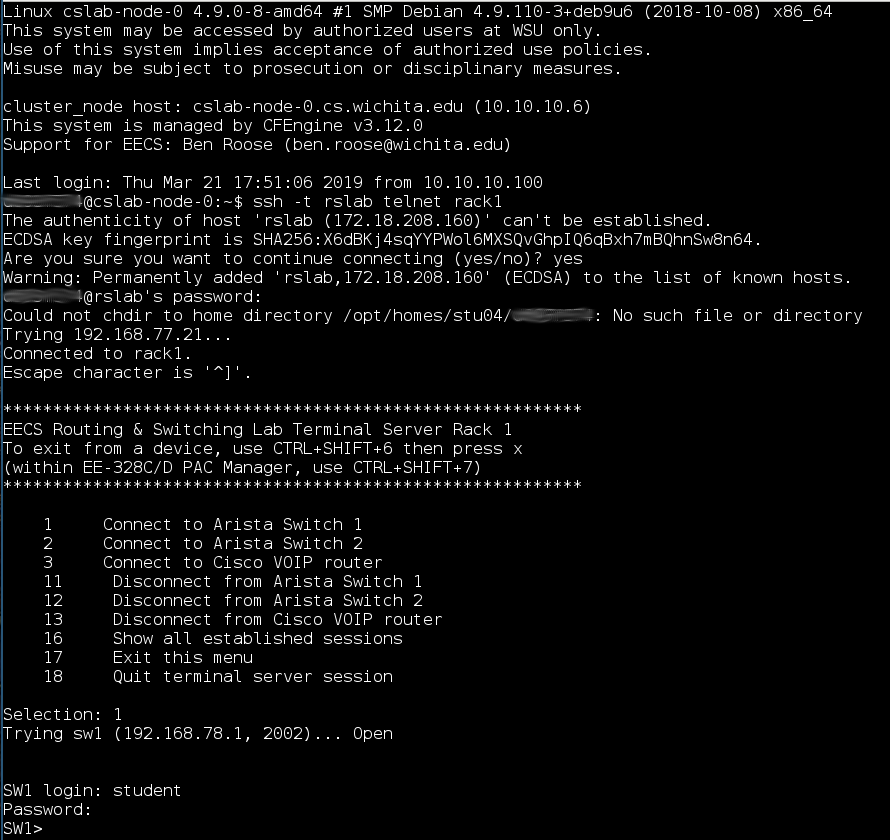
\includegraphics[width=\linewidth]{rslab_ssh_from_cslab}
\centering
\end{figure}

%------------------------------------------------

%% \question{How do I access rslab equipment on Linux or Mac OSX using SSH via cslab-bastion?}\label{remote_access}

%% \begin{enumerate}
%%   \item Follow the \href{https://github.com/benroose/tutorials/blob/master/cslab_tutorials/eecs_tutorial_cslab_ssh_access.pdf}{eecs\_tutorial\_cslab\_ssh\_access} document to configure your SSH client for access into cslab.
%%   \item Copy the following host entries into your local  \verb|~/.ssh/config| file:
%% \end{enumerate}
%% \begin{verbatim}
%% Host rslab rslab.cs.wichita.edu
%%   ProxyCommand ssh your_mywsu_id@cslab-bastion.cs.wichita.edu -W %h:%p
%%   User your_mywsu_id
%%   Compression yes
%%   HostKeyAlias cslab.cs.wichita.edu
%% \end{verbatim}
%% (Ensure to replace \verb|your_mywsu_id| with your own lowercase 8 character myWSU ID number in all three \texttt{ProxyCommand} and \texttt{User} lines.)

%% \begin{enumerate}
%%   \setcounter{enumi}{3}

%%   \item Once logged into cslab \textit{guacamole}, open a \textbf{cslab\_SSH\_CLI\_terminal} connection.
%%   \item Connect to an rslab networking rack, by typing \break
%%     \verb|ssh -t rslab telnet rack#| \break
%%     (where \texttt{\#} is the rack number assigned to you by the lab GTA)
%% \item Enter your myWSU password when prompted to do so.
%% \item You may see a "\texttt{Could not chdir...}" error message when you open a connection to the rslab proxy server. Disregard this message. rslab does not need access to your user home directory for access to the network rack in EE 328D.
%% \item Once connected to the terminal server for your assigned rack, use the menu to connect/disconnect the Arista switches and Cisco router in the networking rack.
%% \item You can return to the terminal server menu by pressing \texttt{CTRL+SHIFT+6} and then \texttt{x}.
%% \item To view all open connections in the session, return to the menu and press \texttt{16}.
%% \item To exit from the terminal server and close the remote SSH connection to the rslab proxy server, return to the menu and press \texttt{18}.
%% \end{enumerate}
%% \textbf{NOTE:} You can open multiple command-line/shell windows from your client machine to access the same rack terminal server and connect to multiple network devices concurrently, but each switch or router can only be accessed by one terminal server session at a time. You can also use a terminal multiplexer such as \textit{tmux} or \textit{screen} within any of the EECS Linux servers to open multiple, simulaneous SSH sessions to an rslab terminal server.

%------------------------------------------------

\question{What do I do if I cannot access the cslab Linux environment? }\label{cslab_problems}
\begin{itemize}
  \item If you cannot access the cslab environment, ensure you have changed your myWSU password within the last three months and can access the myWSU main website \href{https://mywsu.wichita.edu}{mywsu.wichita.edu}. If you cannot access the myWSU website, then you will need to change your password before gaining access into the cslab environment.
  \item If you can access myWSU but cannot access the cslab environment, please contact the EECS systems administrator, \href{mailto:ben.roose@wichita.edu}{ben.roose@wichita.edu}.
\end{itemize}
 
%------------------------------------------------
\newpage

\question{Why do I sometimes see "\texttt{\% Connection refused by remote host}"? }\label{connection_refused}
\begin{itemize}
  \item Though you can open multiple connection sessions to the terminal server controlling each rack, you can only access each network switch or router device within the rack from a single terminal server session.
  \item This access restriction is caused by limitations of the serial communication protocol between the terminal server and each network device in the rack. The access restriction also acts as a security failsafe, since it reduces the possibility of more than one person or lab group attempting to make changes to a switch or router configuration concurrently.
  \item If you see the "\texttt{\% Connection refused by remote host}" error, then either you already have opened a connection to this network device in another terminal server session or another person/lab group has an open connection to this network device. Check you do not already have an open connection in another terminal server session first, then speak with the lab GTA if you cannot resolve the connection refused error yourself.
\end{itemize}

%------------------------------------------------

\question{How do I create a screenshot of my lab session?}\label{screenshot}

\subsection*{EE 328C Linux Terminals}
Within the EE 328C mobile Linux terminals there are three screenshot tools: pressing \texttt{Print Screen} key, using \textit{Take Screenshot} located on the Desktop, or using \textit{PAC Manager's} \textbf{Take Screenshot} menu option.

\subsection*{Remote Access Clients}
Most Windows, Linux and Mac client systems have screenshot tools, which can be used to screenshot the remote access terminal window. Please see your system's documentation for further help.

\newpage
%------------------------------------------------

\question{How do I create a text log of my entire lab session?}\label{logging}

\subsection*{EE 328C Linux Terminals}
Within the EE 328C Linux terminals, \textit{PAC Manager} can log all session data to a text file.
\begin{enumerate}
\item Right-click on the session title tab and select \textbf{Save session log...} from the menu.
\item Enter a name for the log file and click \textbf{Enter} button to save.
\end{enumerate}

\subsection*{Remote Access Clients: Windows computer in lab}
When accessing the rslab remotely with PuTTY on a Windows client, a session log can be specified at the start of the remote SSH session by configuring PuTTY's logging function:
\begin{enumerate}
\item In the \textit{PuTTY Configuration} window, click on \textbf{Logging} category on the left.
\item Select \textbf{All session output} and click on \textbf{Browse} button.
\item Enter a name for the log file and click \textbf{Save} button to save.
\item \textit{Optional:} Logging options can be saved as part of a host connection session in the \textit{PuTTY} \textbf{Saved Sessions} list.
\item For further help on configuring logging in \textit{PuTTY}, see:\\ 
\href{https://the.earth.li/~sgtatham/putty/0.71/htmldoc/Chapter4.html#config-logging}{PuTTY User Manual: Section 4.2}
\end{enumerate}

\subsection*{Remote Access: cslab Linux Environment}
When accessing the rslab remotely from a \textbf{cslab\_SSH\_CLI\_terminal} connection, a session log can be specified at the start of the remote SSH session by typing (where \texttt{\#} is the rack number assigned to you by lab GTA and log\_filename is the path and filename for log) \break
\verb!ssh -t rslab telnet rack# | tee log_filename!

\smallskip

For example: \break
\verb!ssh -t rslab telnet rack1 | tee cs764_assign1.log!

\bigskip

For details on how to download the log file from the cslab Linux environment to your local computer, refer to the \href{https://github.com/benroose/tutorials/blob/master/cslab_tutorials/eecs_tutorial_cslab_web_access.pdf}{eecs\_tutorial\_cslab\_web\_access} document.





%----------------------------------------------------------------------------------------
\newpage
\question{Why is \textit{PuTTY} or \textit{OpenSSH} asking to confirm the authenticity of rslab host keys?}\label{host_keys}

\begin{itemize}
  \item SSH host keys are essential to securing an SSH connection into a remote server. If you see an incorrect host key, then it may mean a cyber-attacker has attempted to compromise the remote server using a ``man-in-the-middle'' attack.
  \item You can manually add SSH host keys to your \textit{PuTTY} and \textit{OpenSSH} known hosts. When adding new host keys you should always ensure the host key fingerprint is correct. \verb|rslab| host key fingerprints must match one of the following SHA256 or MD5 hashes before you add or accept the host key:
\begin{verbatim}
ECDSA key fingerprint is
SHA256:X6dBKj4sqYYPWol6MXSQvGhpIQ6qBxh7mBQhnSw8n64
MD5:d8:ba:c6:1c:86:fa:7f:f6:92:4f:c1:02:30:ce:ab:99

ED25519 key fingerprint is
SHA256:zzozIV7cP1T9C77PLRaevzdzCu21k44lbjd8jaJKS8Q
MD5:6d:3d:8e:3a:db:f6:de:33:af:77:01:40:f3:71:1d:14

RSA key fingerprint is
SHA256:0CUyGZAYMdOd8vTOK3AtM2XTX3lMaGA2NP73rR7s6Ns
MD5:75:5a:16:53:1a:7c:c2:4b:99:66:2d:e3:1e:76:f9:c9

DSA key fingerprint is
SHA256:7zW122xr+aoBb5yiRI96nvdx8Ml07qLKHYwG2Wu6jIM
MD5:27:59:53:18:5a:67:71:f6:32:f1:e1:15:e9:e5:fe:b1
\end{verbatim}

\end{itemize}

%------------------------------------------------

\end{flushleft}
\end{document}
